%%This is a very basic article template.
%%There is just one section and two subsections.
\documentclass{article}
\usepackage[latin1]{inputenc} %coding of writteninput %latin1 allows for Umlaute
\usepackage[T1]{fontenc}%vectorized fonts (cm-super package)
\usepackage[german]{babel}%some specifics of the german language
\usepackage{amsfonts, amsmath, amsthm, amssymb, mathabx, paralist}
 \setlength{\parindent}{0em} 
  \usepackage{listings}
\usepackage{geometry}
  \geometry{a4paper, top=25mm, left=20mm, right=15mm, bottom=20mm, headsep=10mm, footskip=12mm}
 \usepackage{rotating} 
 %Decisiontree
 \usepackage{tikz,forest}
\usetikzlibrary{arrows.meta}
  
\usepackage{graphicx} 

\usepackage{verbatim}%f�r txt datei

\usepackage{color} %red, green, blue, yellow, cyan, magenta, black, white
\definecolor{mygreen}{RGB}{28,172,0} % color values Red, Green, Blue
\definecolor{mylilas}{RGB}{170,55,241}
\usepackage{pdfpages}
\usepackage[section]{placeins}

\title{Assignment 1}

\begin{document}

\section*{Exerise 1}
\subsection*{a)}
The VC-dimension is 3, because you can shatter all sets of size 3, but it is not
possible to shatter the set $\{+-+-\}$. Like to see in the following picture:

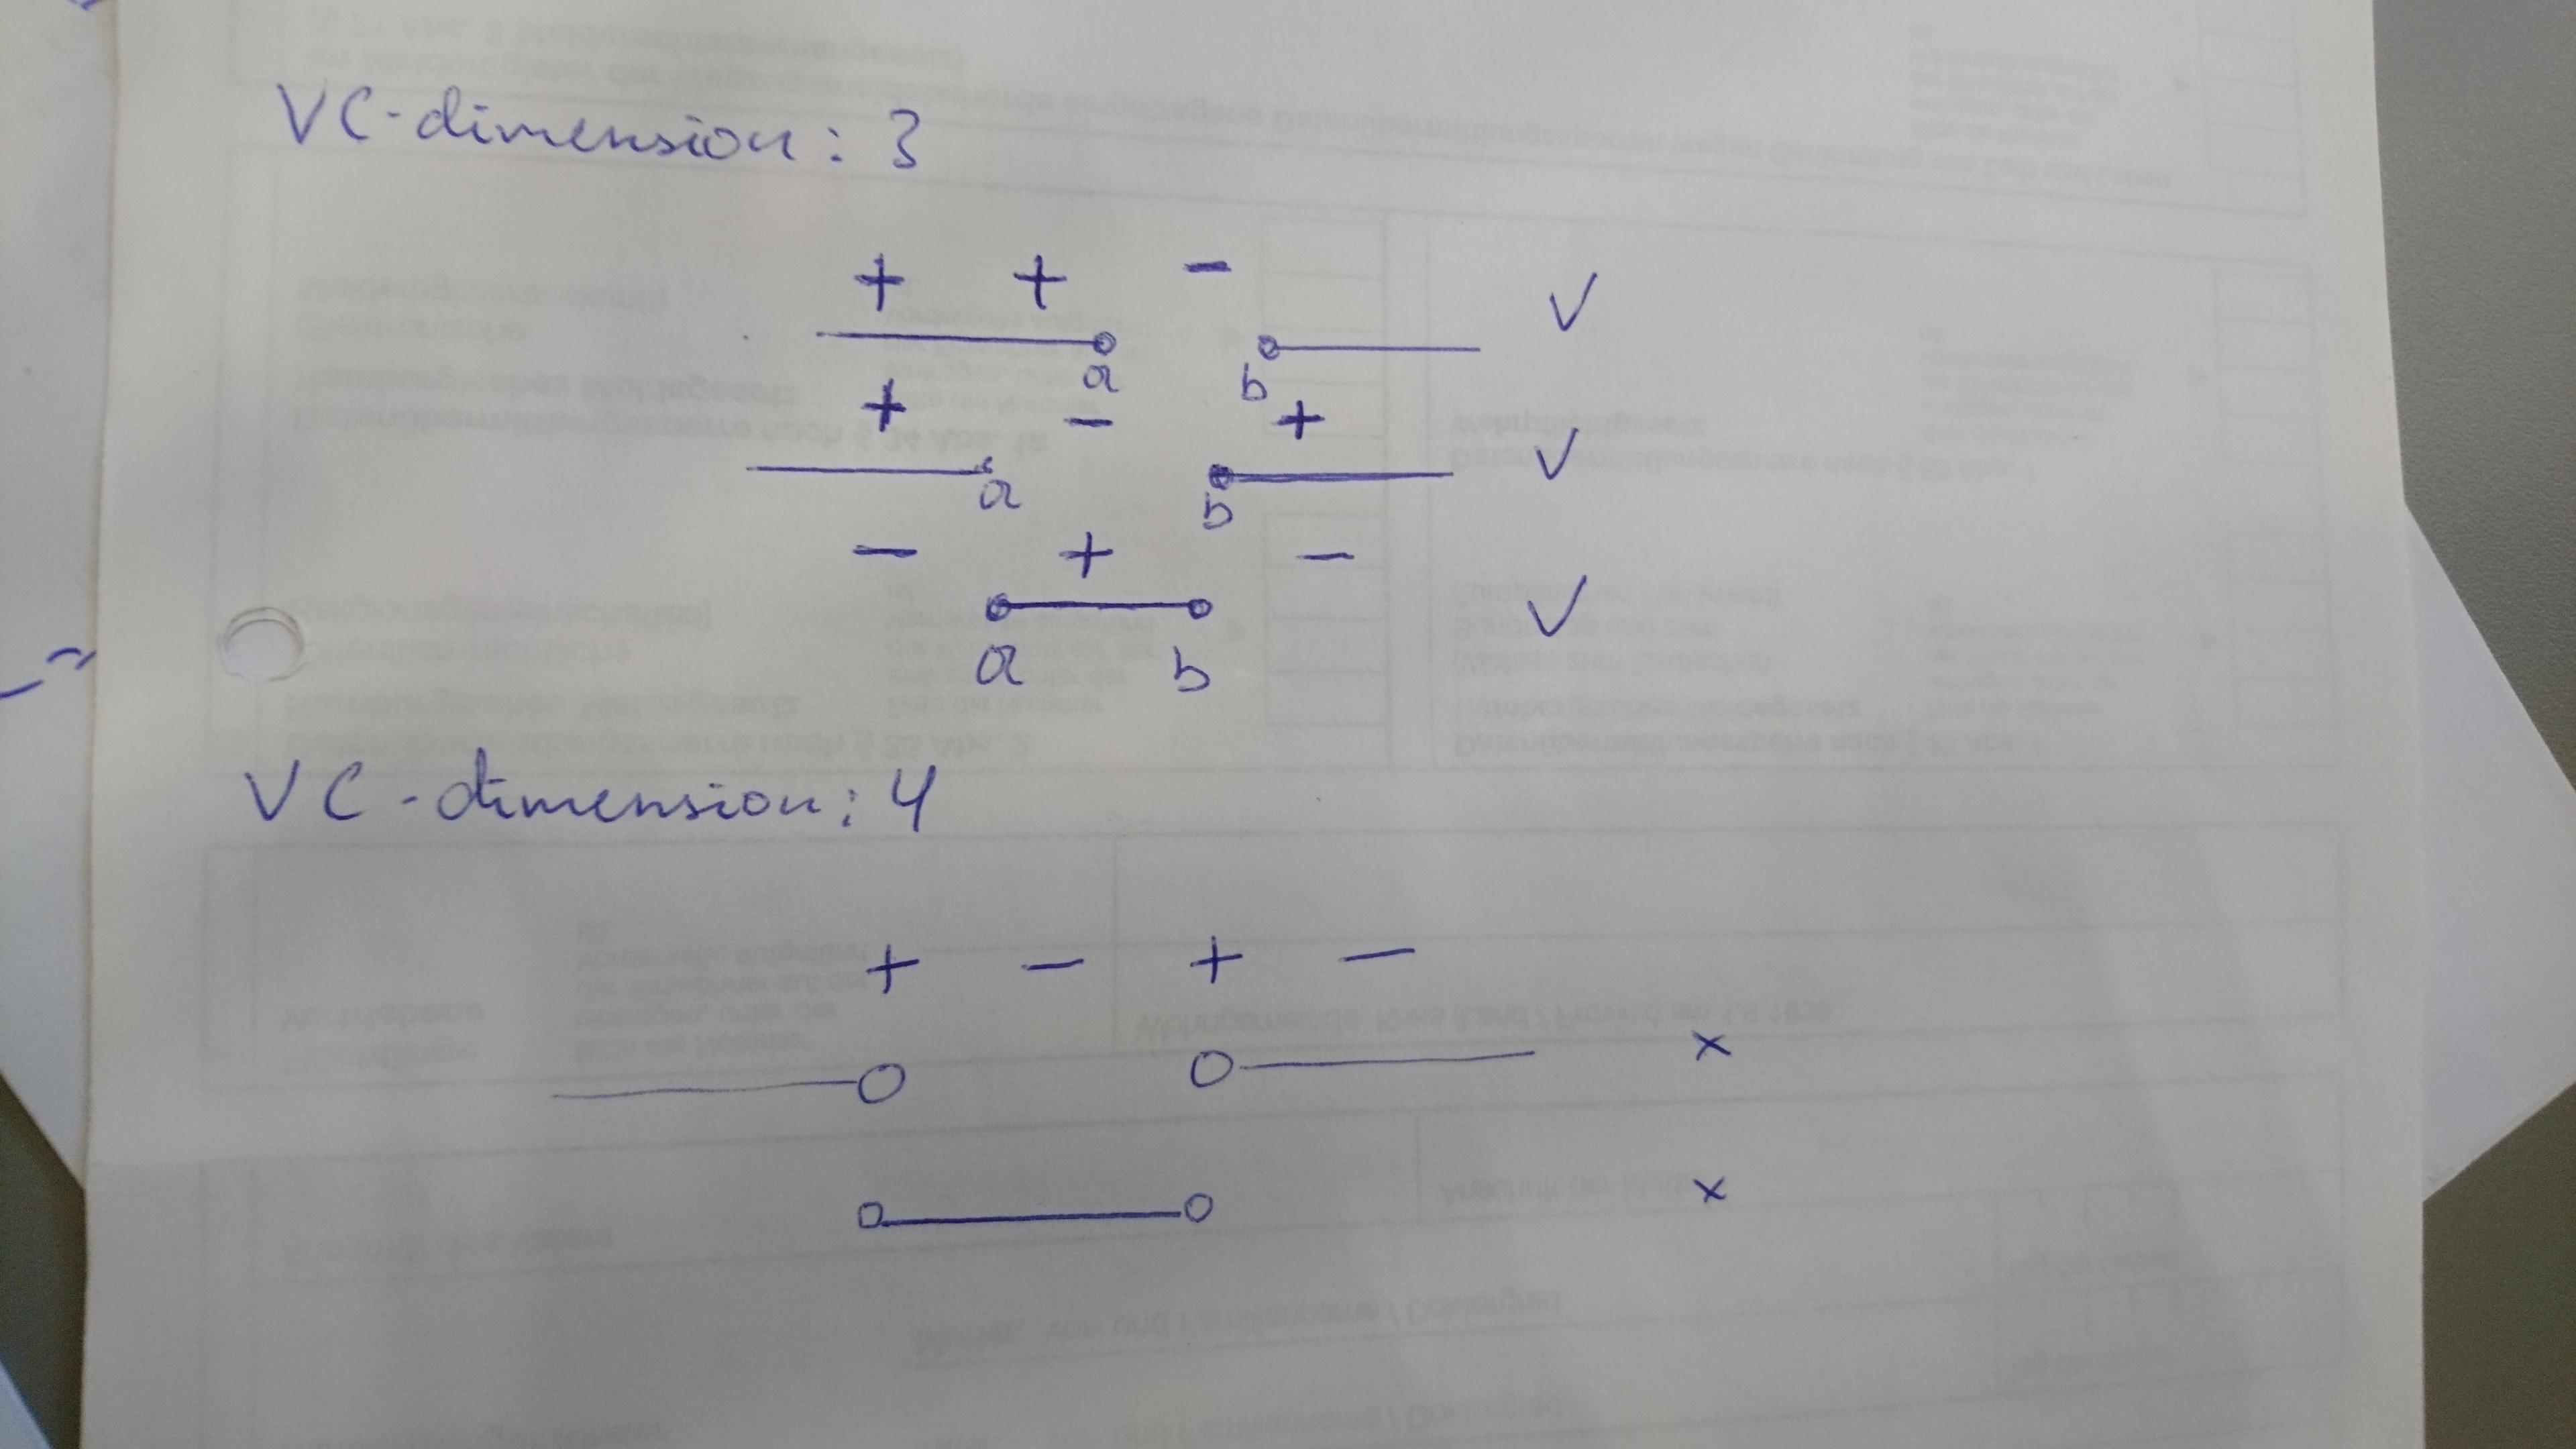
\includegraphics[width=.6\linewidth]{1a.jpg}

\subsection*{b)}

The VC-dimension is $\infty$, 

You construct the set as following:

\begin{enumerate}
  \item All numbers are constructed as product of prime numbers
  \item 
\end{enumerate}
\section*{Exercise 2}
The first observation is, the points have to be in a circle. Wouldn't they be in
a circle, there would always be a point in the middle, that destroys the
shattablilty. The points outside and the point in the middle would have to be of
the same ``classification''.

It is possible to sort 7 points such that they are shattable. Subsets of size 1
and 2 are trivial. All other combinations you can see on the picture.

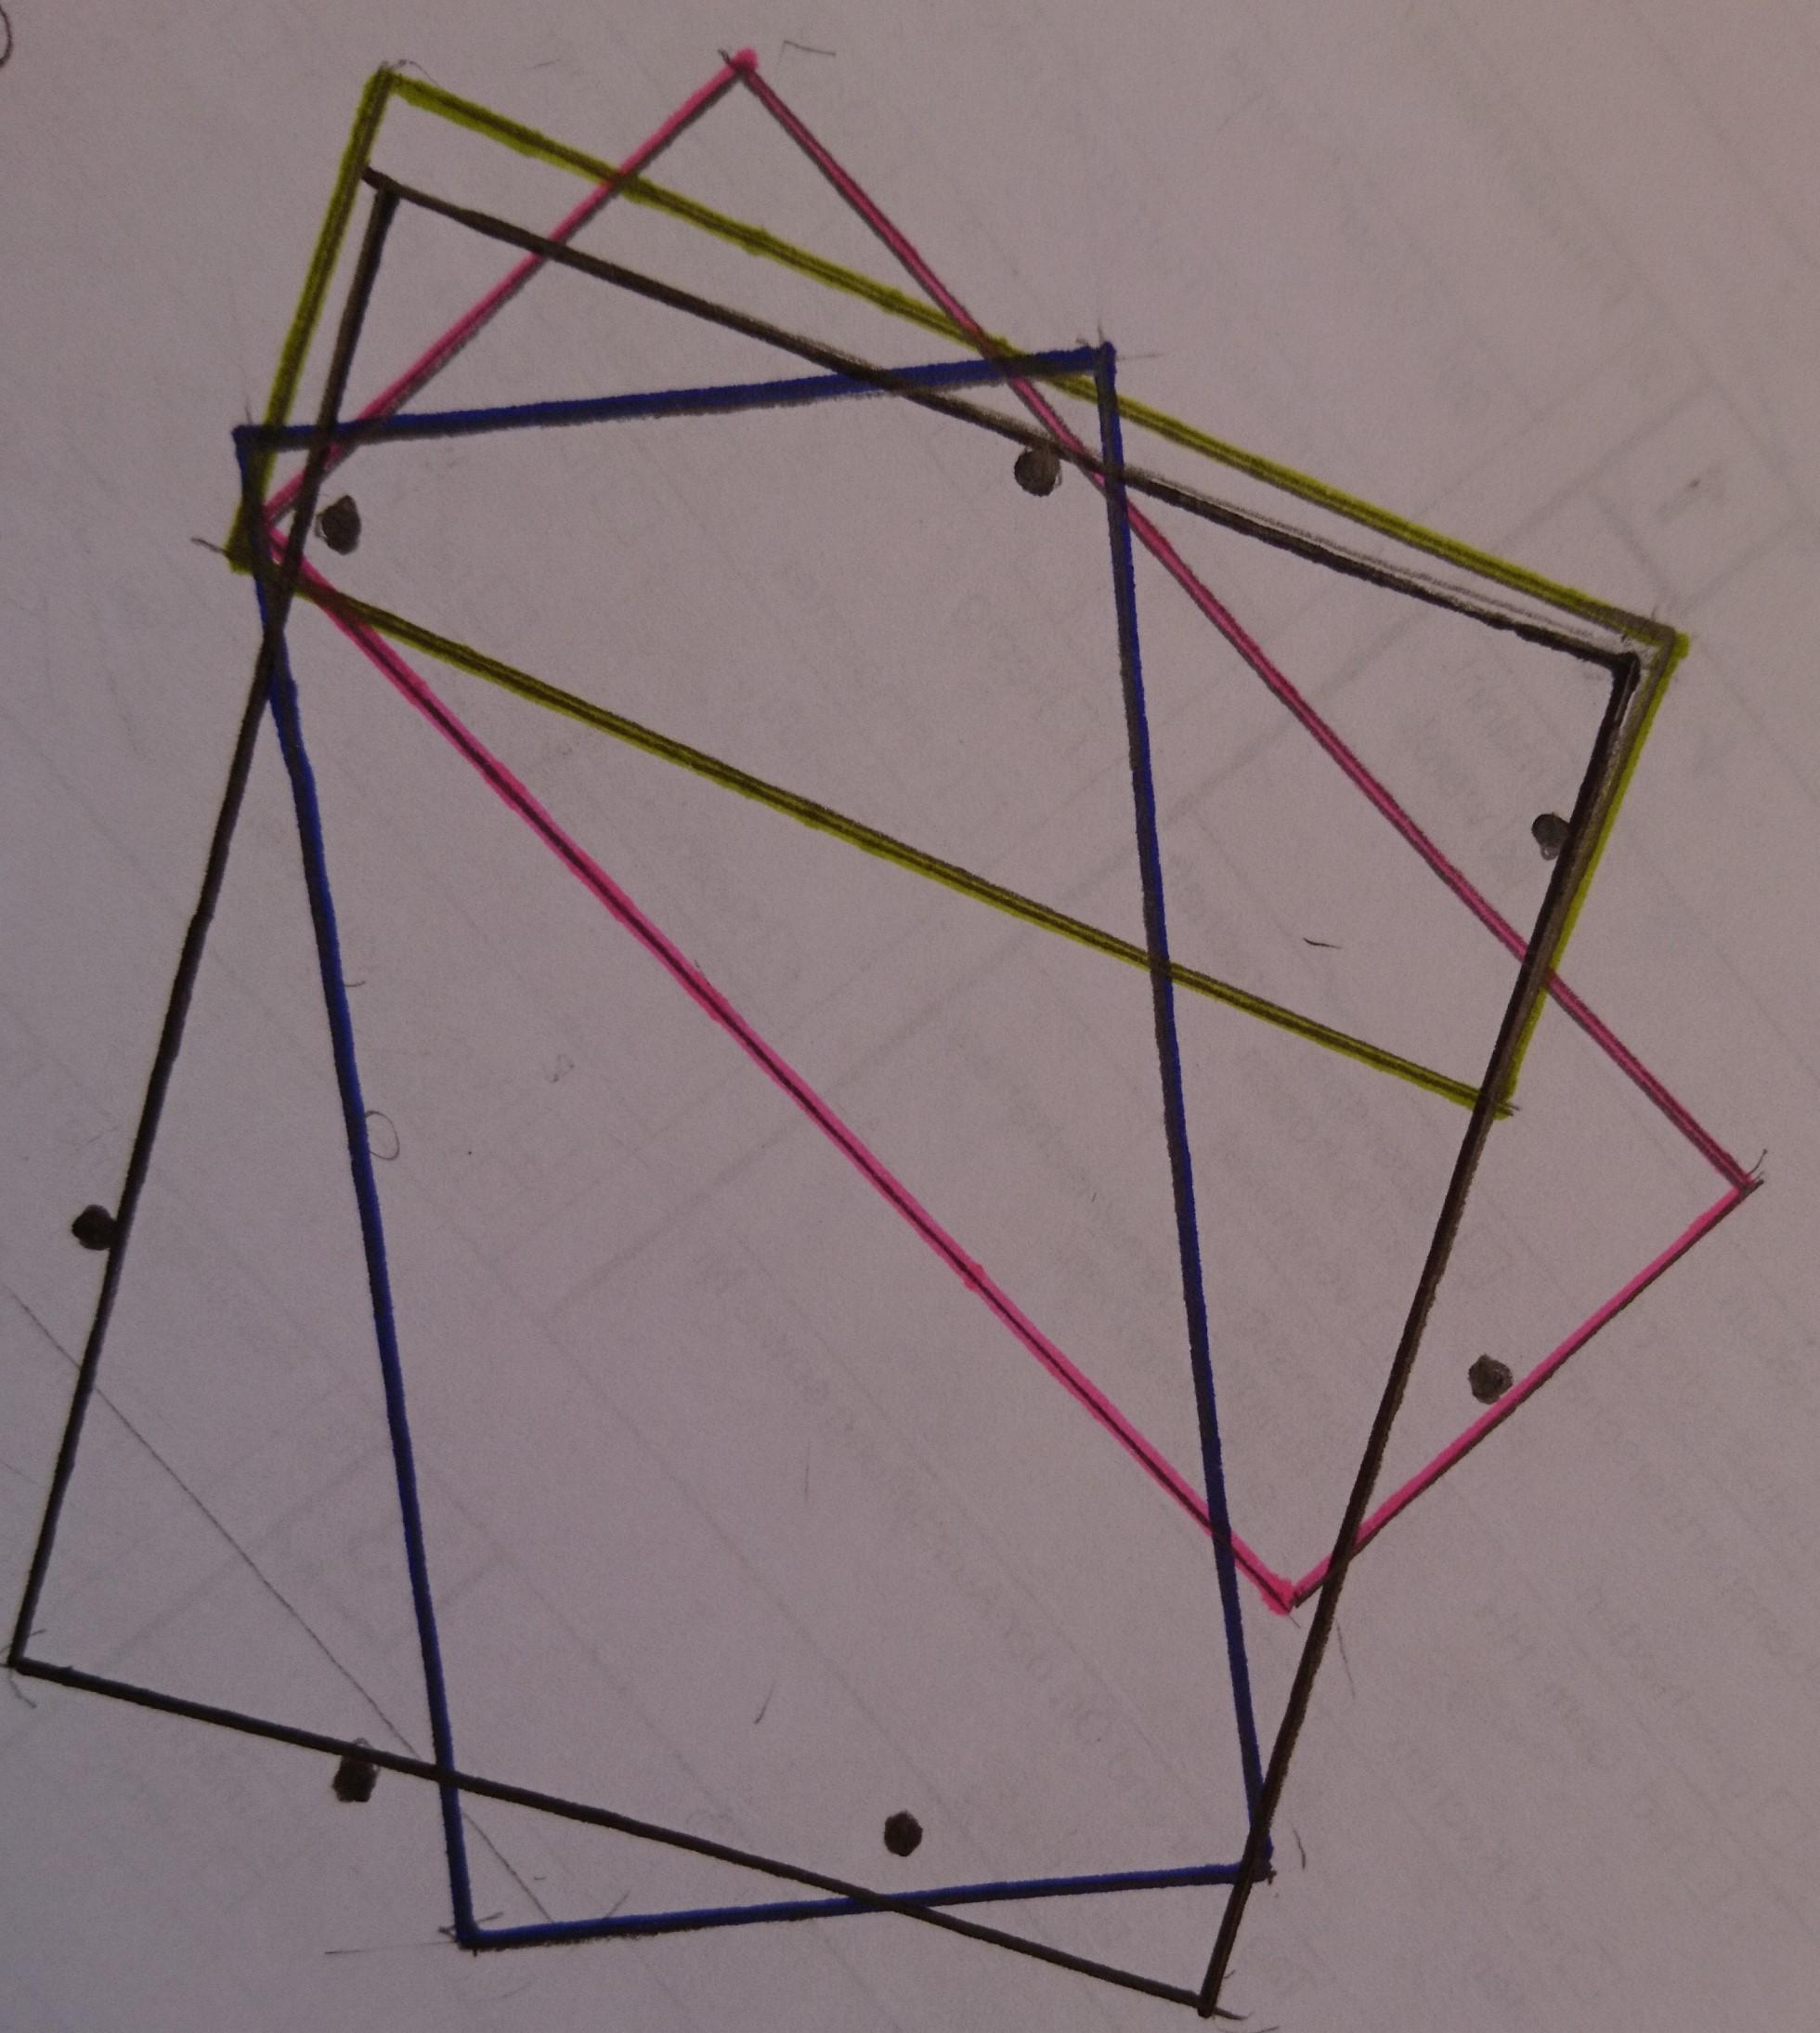
\includegraphics[width=.6\linewidth]{2.jpg}

If you try for 8 points this construction you will fail with a subset of 3. We
know because of the beginning, that they have to be in a ring organized. If you
have that than the following is a counterexample of a subset.

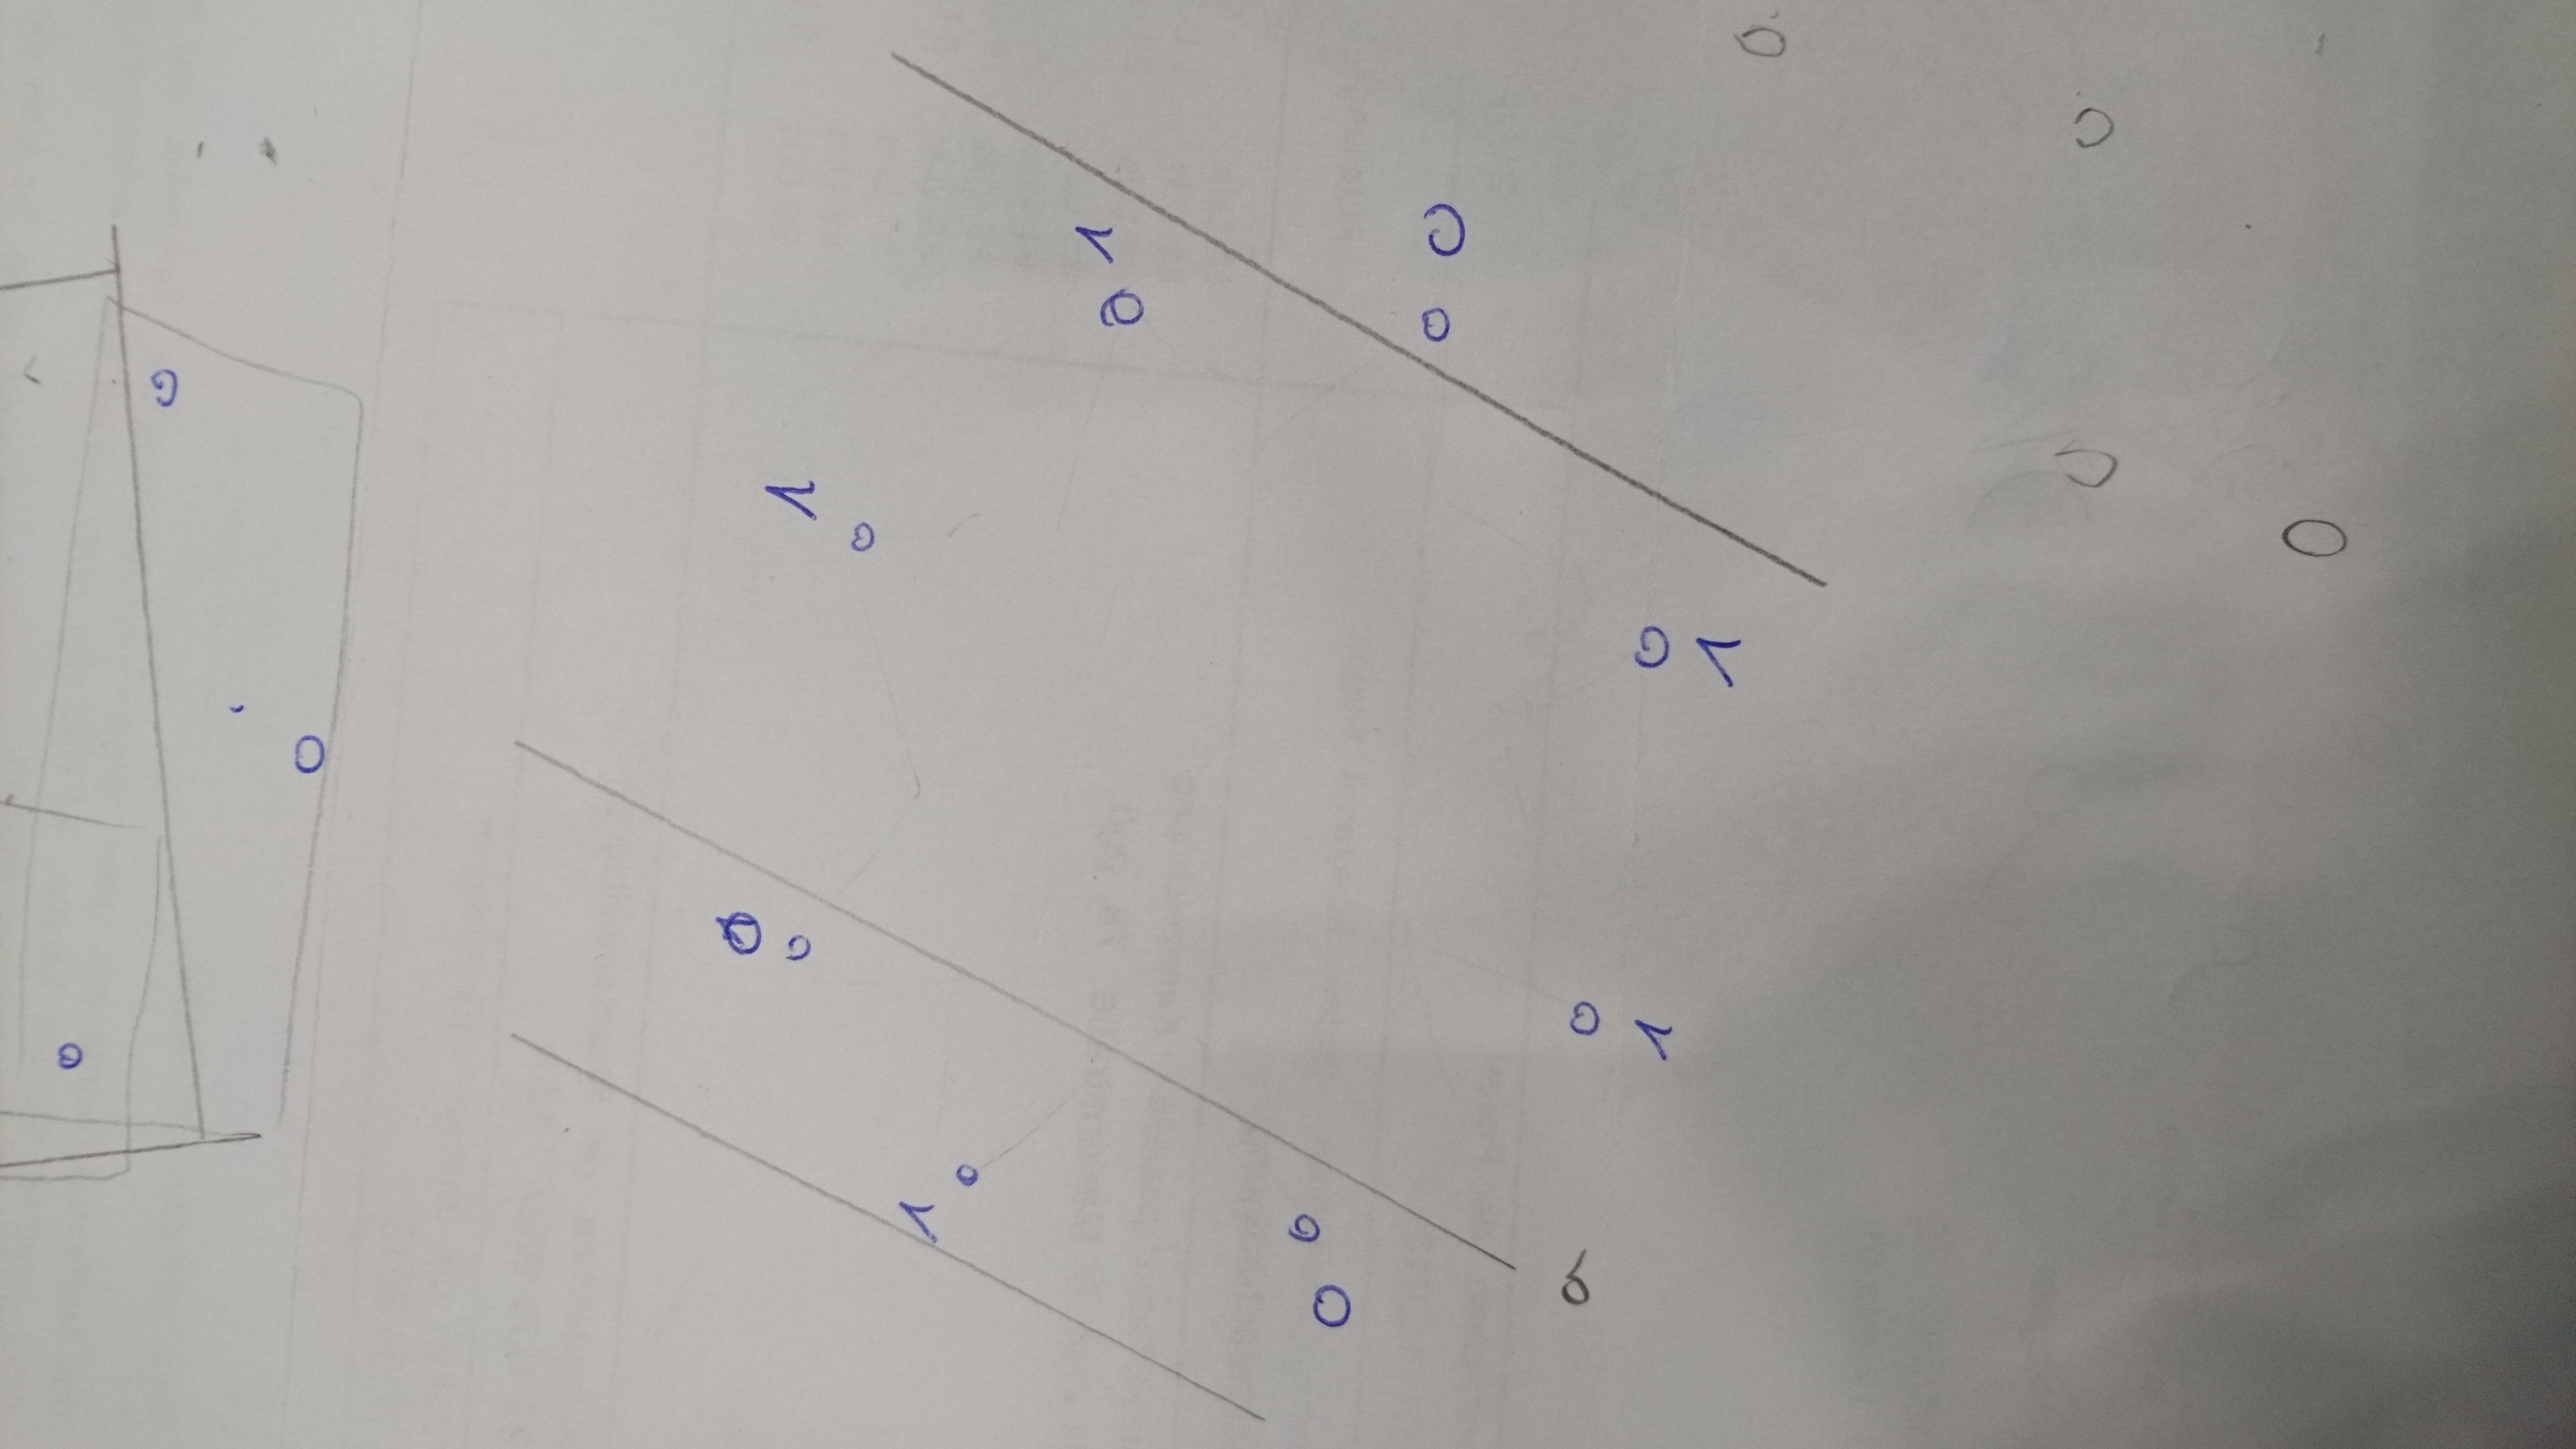
\includegraphics[width=.6\linewidth]{22.jpg}

\end{document}
